\documentclass[10pt]{article}
\usepackage[margin=0.85in]{geometry}
\usepackage{amsmath,amssymb,booktabs,graphicx,caption}
\usepackage[hidelinks]{hyperref}
\captionsetup{font=small}
\setlength{\tabcolsep}{4pt}

\title{Gap versus trial overlap:\\ measured and certified filter cost on $J_1$--$J_2$ chains}
\author{Data report for the filter-pipeline paper}
\date{\today}

\begin{document}
\maketitle

\noindent This report separates the two inputs that set the filter's cost, the spectral gap $\Delta$ and the trial
overlap $\gamma=|\langle E_0|\psi\rangle|^2$. Each is held fixed across system size while the other is varied.
Every \emph{measured} number is an exact state-vector simulation of the Trotterised filter circuit. Every
\emph{certified} number is the pipeline's a-priori bound (Theorem~1) with the same inputs. Nothing is
extrapolated. All tables and figures are generated by \texttt{sbpipe\_study/gapov\_report/make\_report\_gapov.py}
from \texttt{results/gapov\_tune.json} and \texttt{results/gapov.jsonl} (222 cases), produced by
\texttt{sbpipe\_study/run\_gapov.py}.

\section{Holding the gap and the overlap fixed}

\paragraph{Model.} Open $J_1$--$J_2$ Heisenberg chains, $J_1=1$, $N=8,\dots,14$ qubits.
$\Delta=E_1-E_0$ is the singlet--triplet gap from exact diagonalisation.

\paragraph{Gap tuning.} At each $N$, $J_2$ is found by bisection so that $\Delta$ hits the target to $10^{-9}$
(Table~\ref{tab:tune}). The gap closes with $N$ at fixed $J_2$, so larger chains need larger $J_2$. Some
(gap, $N$) pairs have no solution below the dimerised regime and are left out.

\begin{table}[h]\centering\small
\caption{$J_2$ that gives each target gap $\Delta$ at each $N$ (``--'': not reachable).}\label{tab:tune}
\begin{tabular}{ccccc}\toprule
$\Delta$ & $N=8$ & $N=10$ & $N=12$ & $N=14$ \\\midrule
0.30 & -- & -- & 0.4114 & 0.4636 \\
0.35 & -- & 0.4276 & 0.4911 & 0.5135 \\
0.40 & 0.3838 & 0.5101 & 0.5387 & 0.5501 \\
0.45 & 0.5109 & 0.5611 & 0.5755 & 0.5806 \\
0.50 & 0.5762 & 0.6011 & 0.6071 & 0.6083 \\
0.55 & 0.6252 & 0.6359 & 0.6405 & 0.6776 \\
\bottomrule\end{tabular}
\end{table}

\paragraph{Overlap tuning with a real circuit.} The trial is the variational $\chi=16$ MPS, prepared by its
staircase circuit, followed by $R_y(\theta)=e^{-i\theta Y/2}$ on every even site. A uniform rotation on all sites
would do nothing, because the ground state is a singlet and so is invariant under global spin rotations. Rotating
one sublattice breaks that symmetry and lowers $\gamma$ smoothly from the MPS value. $\theta$ is found by
bisection so that $\gamma$ hits the target to $10^{-12}$ (Table~\ref{tab:theta}). The trial cost is the MPS circuit
plus $N/2$ single-qubit rotations, and is the same at every $\gamma$ for a given $N$.

\begin{table}[h]\centering\small
\caption{Rotation angle $\theta$ that sets each overlap $\gamma$ (shown at $\Delta=0.40$).}\label{tab:theta}
\begin{tabular}{lcccc}\toprule
$\gamma$ & $N=8$ & $N=10$ & $N=12$ & $N=14$ \\\midrule
0.03 & 1.516 & 1.604 & 1.549 & 1.474 \\
0.1 & 1.280 & 1.325 & 1.273 & 1.208 \\
0.3 & 0.959 & 0.975 & 0.932 & 0.883 \\
0.5 & 0.739 & 0.746 & 0.712 & 0.673 \\
0.7 & 0.536 & 0.538 & 0.512 & 0.484 \\
0.9 & 0.293 & 0.294 & 0.279 & 0.264 \\
\midrule
$\gamma$ of $\chi=16$ MPS ($\theta=0$) & 1.0000 & 1.0000 & 1.0000 & 1.0000 \\
\bottomrule\end{tabular}
\end{table}

\paragraph{Grid.} Study A fixes $\Delta\in\{0.40,0.50\}$ and varies $\gamma\in\{0.03,0.1,0.3,0.5,0.7,0.9\}$.
Study B fixes $\gamma\in\{0.1,0.5\}$ and varies $\Delta$ over 0.30--0.55. Both run at
$\varepsilon\in\{10^{-2},10^{-3},10^{-4}\}$, for 222 cases in total.

\section{How each cost is obtained}

The cost is the expected number of CNOTs per successful (post-selected) run that leaves the state with
infidelity $1-F\le\varepsilon$:
\begin{equation}
C=\frac{C_\text{filter}+C_\text{trial}}{p},
\end{equation}
where $p$ is the success probability ($p\approx\gamma$).

\paragraph{Measured, dyadic SBC.} Spacing $\tau=\pi/(1+\delta)$, where $\delta=\Delta/W$ is the gap in units of the
spectral width $W$. The exact filter (matrix exponentials) is applied to the trial for each ladder $(K,r)$. The
two shortest ladders that reach $\varepsilon$ are kept. Each is then Trotterised with second-order Strang steps,
and the coarsest common step $dt$ at which the full circuit still reaches $\varepsilon$ is found. The cheaper of
the two is reported.

\paragraph{Measured, QETU (reference).} The smallest even Chebyshev degree whose exact filter reaches
$\varepsilon$ is found. The search then looks for the fewest Strang steps per query, or a slightly higher degree
at one step, that still reaches $\varepsilon$ after Trotterisation.

\paragraph{Certified.} The pipeline's \texttt{refine()} with exact energies ($E_0,E_1$ errors $10^{-9}$), the
Weyl upper bound on the spectrum and the true $\gamma$. This gives the circuit that Theorem~1 guarantees
reaches $\varepsilon$ with commutator Trotter bounds, without simulating it.

\section{Study A: gap fixed, overlap varied}

\begin{figure}[h]\centering
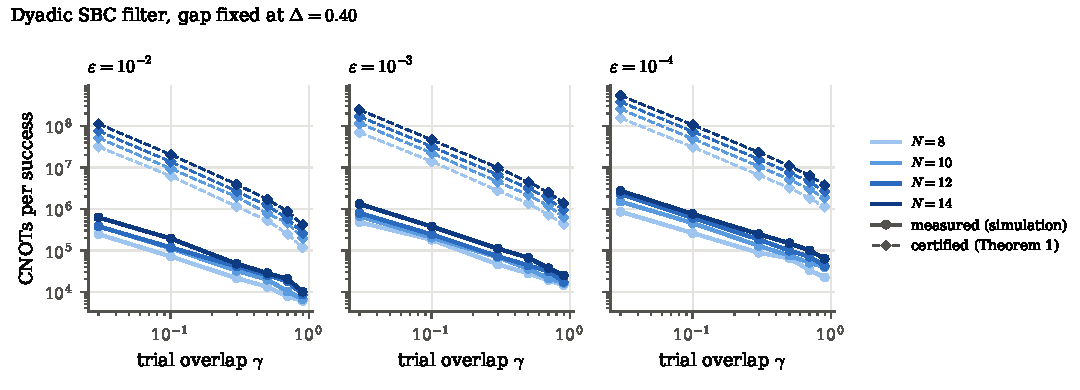
\includegraphics[width=\linewidth]{figs/fig_gapov_A.pdf}
\caption{Dyadic SBC filter at $\Delta=0.40$ for every $N$. Solid: measured by simulation. Dashed: certified.}
\label{fig:A}
\end{figure}

\begin{table}[h]\centering\small
\caption{Dyadic filter at $\Delta=0.40$, $\varepsilon=10^{-3}$: measured / certified CNOTs per success.}
\begin{tabular}{lcccc}\toprule
$\gamma$ & $N=8$ & $N=10$ & $N=12$ & $N=14$ \\\midrule
0.03 & $2.6\times10^{5}$ / $3.3\times10^{7}$ & $3.6\times10^{5}$ / $5.6\times10^{7}$ & $4.5\times10^{5}$ / $8.2\times10^{7}$ & $7.2\times10^{5}$ / $1.2\times10^{8}$ \\
0.1 & $9.5\times10^{4}$ / $6.6\times10^{6}$ & $1.1\times10^{5}$ / $1.1\times10^{7}$ & $1.4\times10^{5}$ / $1.5\times10^{7}$ & $2.1\times10^{5}$ / $2.3\times10^{7}$ \\
0.3 & $2.5\times10^{4}$ / $1.3\times10^{6}$ & $3.8\times10^{4}$ / $2.2\times10^{6}$ & $4.1\times10^{4}$ / $3.2\times10^{6}$ & $6.2\times10^{4}$ / $4.8\times10^{6}$ \\
0.5 & $1.5\times10^{4}$ / $6.5\times10^{5}$ & $2.0\times10^{4}$ / $1.0\times10^{6}$ & $2.5\times10^{4}$ / $1.5\times10^{6}$ & $3.7\times10^{4}$ / $2.2\times10^{6}$ \\
0.7 & $1.0\times10^{4}$ / $3.4\times10^{5}$ & $1.2\times10^{4}$ / $5.6\times10^{5}$ & $1.8\times10^{4}$ / $8.4\times10^{5}$ & $2.1\times10^{4}$ / $1.2\times10^{6}$ \\
0.9 & $7.9\times10^{3}$ / $2.0\times10^{5}$ & $9.5\times10^{3}$ / $3.0\times10^{5}$ & $1.1\times10^{4}$ / $4.6\times10^{5}$ & $1.5\times10^{4}$ / $6.7\times10^{5}$ \\
\bottomrule\end{tabular}
\end{table}

\paragraph{Result.} Overlap is the dominant input. At $\Delta=0.40$, lowering $\gamma$ from 0.9 to 0.03 (a factor
of 30) raises the measured dyadic cost by 33--62$\times$ and the certified cost by 137--273$\times$. Most of the
rise is the repetition $1/p\approx1/\gamma$: each success needs about $1/\gamma$ attempts. The rest comes from the
longer filter needed to remove more excited weight (larger $L$). The curves for different $N$ run nearly parallel,
so the effect of the overlap does not depend on size over this range. Across all cases the certificate lies
14--258$\times$ (median 62$\times$) above the measured dyadic cost. The excess is largest at small $\gamma$, because the bound grows faster in
$L$ than the measured cost does (Table~\ref{tab:fit}).

\section{Study B: overlap fixed, gap varied}

\begin{figure}[h]\centering
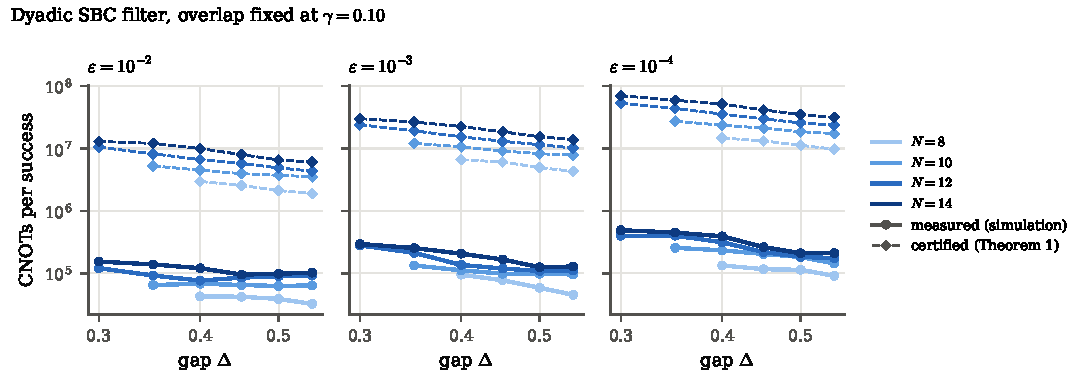
\includegraphics[width=\linewidth]{figs/fig_gapov_B.pdf}
\caption{Dyadic SBC filter at $\gamma=0.10$ with the gap held fixed across $N$. Solid: measured. Dashed: certified.}
\label{fig:B}
\end{figure}

\paragraph{Result.} At fixed overlap, the gap matters much less over the range that can be held fixed at every
$N$. At $\gamma=0.1$, closing $\Delta$ from 0.55 to 0.30 (a factor of 1.8) raises the measured dyadic cost by
1.1--2.9$\times$, QETU by 1.4--1.8$\times$ and the certified cost by 1.5--2.4$\times$. At fixed $\Delta=0.40$ and
$\gamma=0.1$, growing the chain from $N=8$ to 14 raises the measured cost 2.1--2.9$\times$ and the certified cost
3.3--3.4$\times$. A wider gap range is not reachable at every $N$ (Table~\ref{tab:tune}), so the gap exponent is
less well pinned than the overlap one.

\section{Cost as a function of $N$, $\Delta$, $\gamma$ and $\varepsilon$}

Every case, from both studies and all three $\varepsilon$, is fitted to one form:
\begin{equation}\label{eq:fit}
C\;\approx\;a\,N^{\alpha}\,\Delta^{-\beta}\,L^{\lambda}\,\gamma^{-g},\qquad
L=\ln\frac{1-\gamma}{\gamma\,\varepsilon}.
\end{equation}
$L$ is the log factor every filter needs: to bring infidelity from $(1-\gamma)/\gamma$ down to
$\varepsilon$, it must suppress the excited weight by $\eta^2=\gamma\varepsilon/(1-\gamma)$.

\begin{table}[h]\centering\small
\caption{Fitted exponents of Eq.~\eqref{eq:fit}, using every case. ``rms'' and ``max'' are the typical and worst
factor by which a case differs from the fit.}\label{tab:fit}
\begin{tabular}{lcccccccc}\toprule
 & $a$ & $\alpha$ ($N$) & $\beta$ ($\Delta$) & $\lambda$ ($L$) & $g$ ($\gamma$) & rms & max & cases \\\midrule
dyadic, measured & $1.01\times10^{1}$ & 1.50 & 1.15 & 1.41 & 0.78 & 1.23$\times$ & 1.9$\times$ & 222 \\
QETU, measured & $1.31\times10^{1}$ & 2.09 & 0.74 & 0.68 & 0.99 & 1.04$\times$ & 1.2$\times$ & 222 \\
dyadic, certified & $1.50\times10^{1}$ & 2.07 & 1.27 & 2.43 & 0.98 & 1.22$\times$ & 2.2$\times$ & 222 \\
QETU, certified & $9.53$ & 2.03 & 1.11 & 2.17 & 0.99 & 1.22$\times$ & 2.0$\times$ & 222 \\
\bottomrule\end{tabular}
\end{table}

\begin{figure}[h]\centering
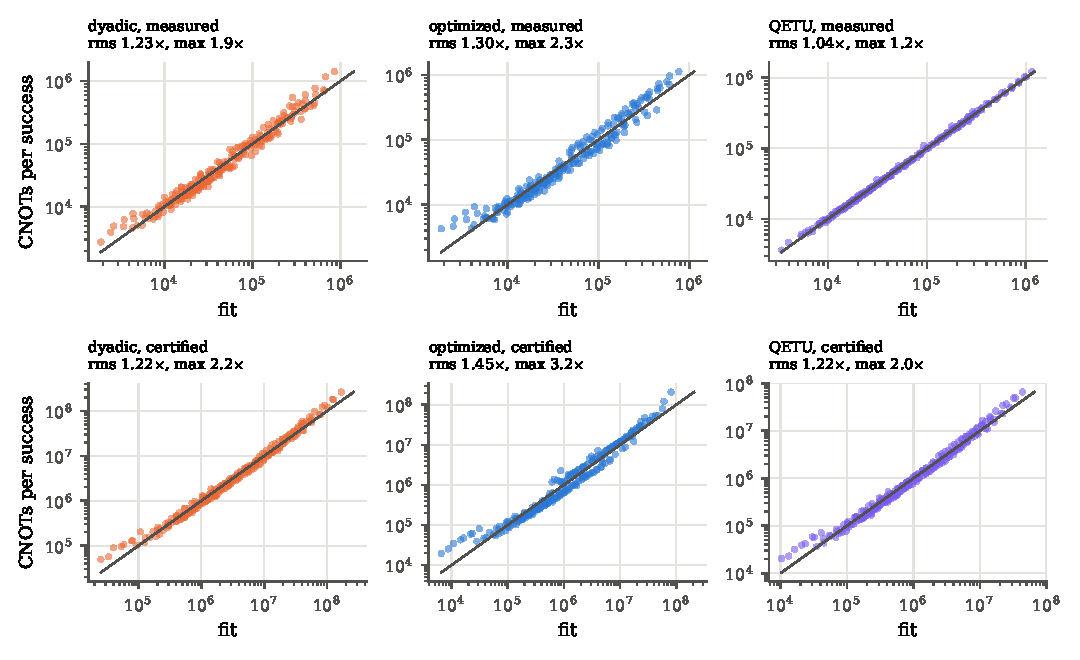
\includegraphics[width=\linewidth]{figs/fig_gapov_fit.pdf}
\caption{Each case against its fit, Eq.~\eqref{eq:fit} with Table~\ref{tab:fit}.}\label{fig:fit}
\end{figure}

\paragraph{The cost rules.} With $L=\ln[(1-\gamma)/(\gamma\varepsilon)]$, the expected CNOTs per success are
\begin{align}
C^{\text{meas}}_{\text{dyadic}}&\approx 1.01\times10^{1}\;N^{1.50}\,\Delta^{-1.15}\,L^{1.41}\,\gamma^{-0.78}
&&(\text{within } 1.23\times\text{ typical, } 1.9\times\text{ worst}),\\
C^{\text{meas}}_{\text{QETU}}&\approx 1.31\times10^{1}\;N^{2.09}\,\Delta^{-0.74}\,L^{0.68}\,\gamma^{-0.99}
&&(1.04\times,\ 1.2\times),\\
C^{\text{cert}}_{\text{dyadic}}&\approx 1.50\times10^{1}\;N^{2.07}\,\Delta^{-1.27}\,L^{2.43}\,\gamma^{-0.98}
&&(1.22\times,\ 2.2\times),\\
C^{\text{cert}}_{\text{QETU}}&\approx 9.53\;N^{2.03}\,\Delta^{-1.11}\,L^{2.17}\,\gamma^{-0.99}
&&(1.22\times,\ 2.0\times).
\end{align}
Three of the four rules have $\gamma^{-1}$ almost exactly, which is the post-selection repetition. The measured
dyadic rule has $\gamma^{-0.78}$, because its success probability ranges from 0.76 to 1.24 times $\gamma$:
the ladders over-suppress, so part of its $\gamma$ dependence is absorbed into $L$. The certified rules grow
as $L^{2.2\text{--}2.4}$, where the measured ones grow as $L^{0.8\text{--}1.7}$. That difference is why the
certificate's overhead grows at small $\gamma$ and small $\varepsilon$. The certified $N^{2}$ is one factor of
$N$ from the CNOTs per Trotter step and one from the spectral width $W\propto N$, which sets the filter length at a
fixed gap.

\paragraph{Dyadic versus QETU, measured.} Over all cases, QETU costs a median 1.26$\times$ the dyadic filter.
The dyadic filter is cheaper in every case at $\varepsilon=10^{-2}$ and in all but 9 at $10^{-3}$. At
$\varepsilon=10^{-4}$ QETU is cheaper in 56 of 74 cases, because the dyadic ladder lengthens in coarse
power-of-two steps. The fits show the same thing: the dyadic cost grows as $L^{1.41}$ against $L^{0.68}$ for
QETU, while the dyadic cost grows more slowly with $N$ ($N^{1.50}$ against $N^{2.09}$).

\section{Caveats}
\begin{itemize}
\item The sizes span $N=8$--14 (less than a factor of two), and the gaps span 0.30--0.55. The exponents
summarise these data. They are not asymptotic laws, and the $N$ exponent in particular is loose.
\item The $N$ exponent mixes two effects: the CNOTs per Trotter step (about $\propto N$) and the spectral width
$W\approx0.7N$, which sets the filter length at a fixed gap in absolute units.
\item The certified fit summarises the bound over this grid. The bound itself (Theorem~1) holds case by case
and does not depend on the fit.
\item The dyadic filter is discrete: $(K,r)$ and $dt$ move in jumps, so its measured cost scatters more about
the fit than QETU's does.
\end{itemize}

\end{document}
